\documentclass[12pt,twoside,openany]{report}
\usepackage[T1]{fontenc}
\usepackage[utf8]{inputenc}
\usepackage[english]{babel}

\usepackage[backend=biber,style=authoryear-ibid]{biblatex}
\usepackage{csquotes}
\addbibresource{references.bib}

\usepackage[a4paper]{geometry}
\usepackage{fancyhdr}
\pagestyle{fancy}

\usepackage{hyperref}

\usepackage{titlesec}

\titleformat{\chapter}
  {\Large\bfseries} % format
  {}                % label
  {0pt}             % sep
  {\huge}           % before-code

\usepackage{graphicx}
\graphicspath{{images/}}
\usepackage{float} % to use H option

% loading in math packages
\usepackage{mathtools}
\usepackage{amsmath}
\usepackage{amssymb}
\usepackage{siunitx}
\usepackage{gensymb}

\usepackage[version=4]{mhchem}

\begin{document}

%\maketitle

\begin{titlepage} 
\newcommand{\HRule}{\rule{\linewidth}{0.5mm}} 
	  
\center % Centre everything on the page

%------------------------------------------------
% Headings
%------------------------------------------------
\textsc{\textbf{\LARGE Università degli Studi di Trento}}\\[1.5cm] 
		 
		   
\textsc{\textbf{\Large Dipartimento di Fisica }}\\[0.5cm] 
		     
%------------------------------------------------
% Title
%------------------------------------------------

\HRule\\[0.4cm]
	
{\huge\bfseries XY model}\\[0.1cm] % Title of your document

\HRule\\[1.5cm]

\vfill
\begin{figure}[h]
\centering
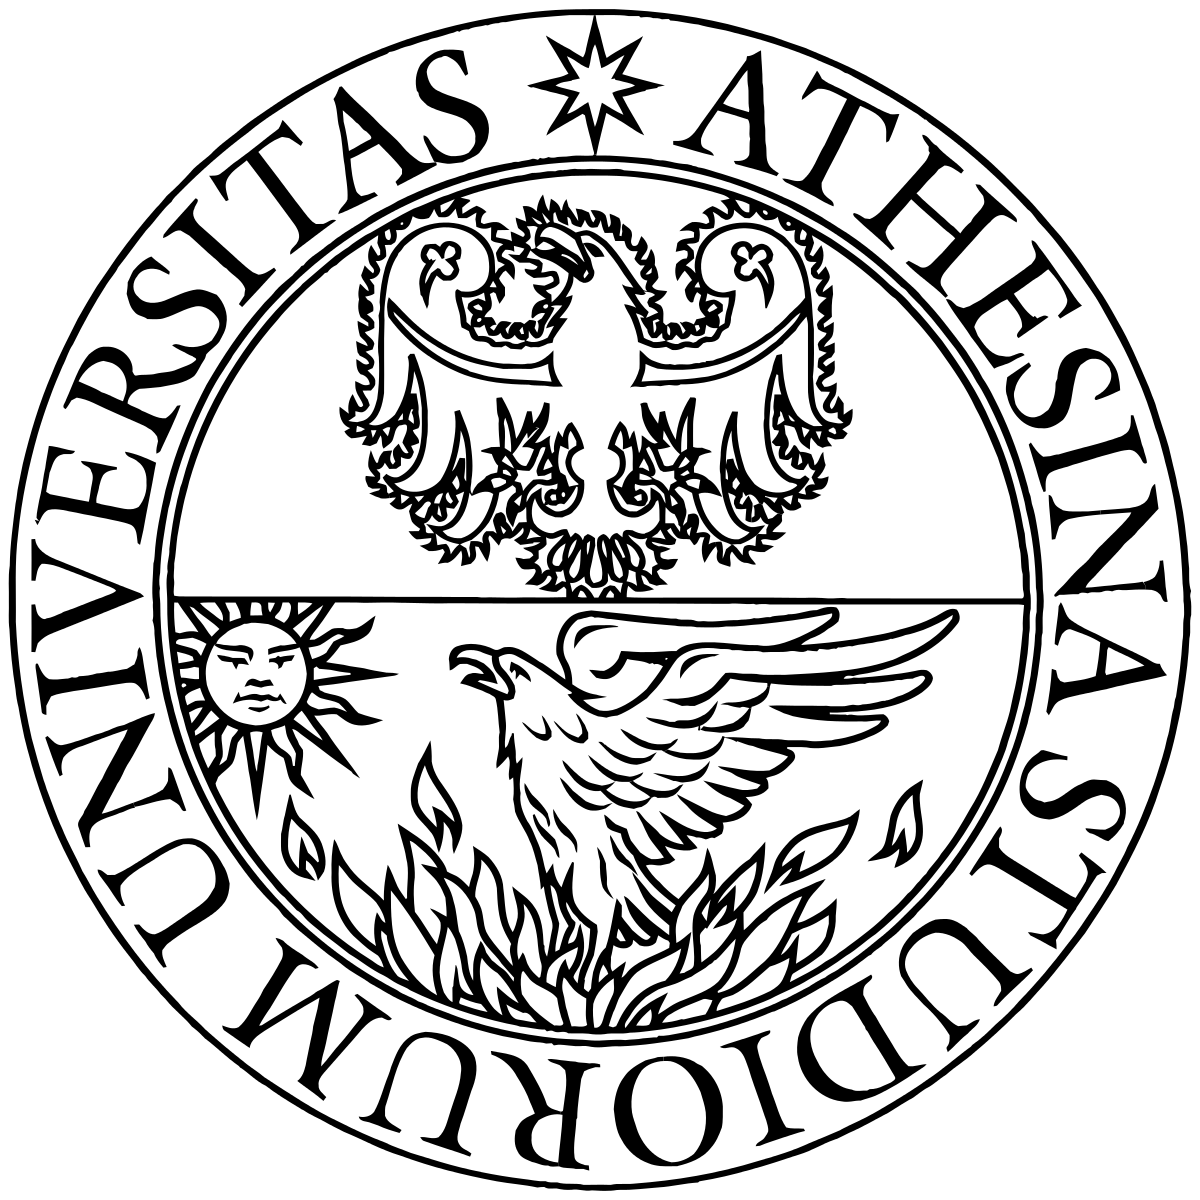
\includegraphics[scale=0.18]{logo.png}
\end{figure}

\vfill

\begin{figure}[h]
\centering
\begin{minipage}{0.4\textwidth}
			    
\Large
\textbf{\textit{Author}\\
	Francesco\\ \textsc{Musso}} % Author's name

\end{minipage}
\qquad \qquad \qquad
\begin{minipage}{0.4\textwidth}

\begin{flushright}
\Large
\textbf{\textit{Supervisor}\\
	Prof. Francesco \textsc{Pederiva}} % Supervisor's name
\end{flushright}

\end{minipage}
\end{figure}

\vfill
\textbf{{\Large November 2020}}

\end{titlepage}

\tableofcontents

\chapter{Introduction}
\section{Lattice models for phase transitions}

A very successful and general set of models in statistical mechanics is the
one in which the components of a system are located on an array of lattice sites,
with every component interacting only with the closest ones
(\emph{nearest-neighbour interaction}).
This kind of models turns out to describe well enough a very broad range of phase 
transitions including ferromagnetism transitions, gas-liquid and gas-solid 
transitions, superconductive transitions and so on. \footnote{The foregoing
discussion is heavily based on ~\textcite{pathria1972statistical} section 12.3}

The case considered in this dissertation will be the \emph{ferromagnetic}
transitions.

Being defined on a lattice entails a discretization of space, a caveat 
that fits very well if the system under study is a metal whose atoms are almost 
locked in a crystalline structure. The crystalline nature of metals allows to
introduce another semplification in this kind of models: considering the atoms
as harmonic oscillators swinging around the equilibrium point, their kinetic energy can 
be neglected and only their magnetic interactions has to be considered. 
It has to be said that this kind of facilitation turns out to be 
adequate also for other kinds of transitions and for materials very different 
from metals.

\section{Hamiltonian of ferromagnetic lattice systems}

Being interested only in the magnetic interactions of atoms means that they can be considered as 
magnetic dipoles having a magnetic moment $\mathbf{\mu}$. Every magnetic dipole
in the $N$ lattice sites will have a magnitude $\mu = g \mu_B \sqrt{J(J+1)}$, 
with $g$ being the Landè factor, $\mu_B$ the Bohr magneton and $J$ being the
total angolar momentum quantum number. The total number of possible orientations of
the magnetic momenta in space is given by the multiplicity of $J$: $(2J+1)$. This 
magnetic dipoles will interact witch each other and will interact with an eventual
external field $\mathbf{B}$.

The net magnetization of the system $\overline{M}$ will depend on both the 
temperature $T$ and the field $B$ ($\overline{M} \equiv \overline{M}(T,B)$). 
Studying the \emph{spontaneous magnetization} $\overline{M}(T,0)$ of the system,
a \emph{critical temperature} $T_c$ can be defined as the threshold temperature
for $\overline{M}(T_c,0) \neq 0$ for $T < T_c$: above $T_c$ the thermal agitation 
will be too big to allow a spontaneous magnetization to manifest, then at $T_c$ the
system will perform a \emph{ferromagnetic transition}.

Detailed studies beyond the scope of this dissertation have shown that ferromagnetic
properties arise when $J=\frac{1}{2}$ and so it can be assumed that this kind of 
phenomena are due to electrons' spin. Then the magnetic moment can be rewritten as 
$\mu = 2 \mu_B \sqrt{s(s+1)}$, where $g=2$ is the Landè factor for electrons and
$s$ is the spin of the electron.

From quantum mechanics considerations \parencite[see][]{bransden2003physics}
it can be shown that the interaction energy between two electrons can be expressed
as $K_{ij} \pm J_{ij}$ with $i$ and $j$ being the two indices indicating two
neighbouring electrons. The plus and minus sign are determined based on $S$, the 
total spin of the the two electron: the plus corresponding to the case $S=0$ and 
the minus to one with $S=1$, where only $J_{ij}$ depends on the spins' configuration.

Then the energy difference between the "parallel" spin configuration and the 
"antiparallel" spin configuration is
$$\Delta E = E_{\uparrow\uparrow} - E_{\uparrow\downarrow} = -2J_{ij}$$
Defining the scalar product operator of the spin of the two electron as 
$$ \mathbf{s}_j \cdot \mathbf{s}_i = \frac{1}{2} S(S+1) - s(s+1)$$
is easy to show that the interaction energy between the spins can be written as
$$ E_{ij} = \text{const.} - 2J_{ij} (\mathbf{s}_i \cdot \mathbf{s}_j)$$

The exact value of the constant is irrilevant since any constant can be added to
the potential energy. Still from quantum mechanical considerations it can be seen
that $J_{ij}$ falls very rapidly when the distance beetwen the two spins increases,
supporting our initial caveat of regarding only the neirest-neighbours interactions.


\section{\textit{n}-vector models}

In statistical mechanics the formalization of the ideas presented in the previous
sections for ferromagnetic lattice models is the so called \textit{n}-vector model.
A \textit{n}-vector model is a system of interacting spins on a crystalline lattice 
as the ones described above. This formalization was developed by Stanley
\parencite[see][]{PhysRevLett.20.589} who was able to show that most of the
critical properties of this kind of systems depends only on the dimension of the
lattice and on the dimensionality of the spins in the system.

Fromalized in a mathematical way we have a \textit{n}-vector model when we can 
describe a system composed of \textit{n}-dimensional spins as unit-length vectors,
located on the sites of $d$ dimensional lattice.

The evolution of the system is described by the hamiltonian
\begin{equation}
	H = - J \sum_{n.n.} \mathbf{s}_i \cdot \mathbf{s}_j
	\label{eq:ham_nvector}
\end{equation}
where the meaning of the symbols follows directly from the one used in the
previous sections and the subscript $n.n.$ means the summation goes over only
on the nearest-neighbour spins. 

Equation~\ref{eq:ham_nvector} shows that \emph{ferromagnetic} phenomena are  
possible when $J > 0$ since the configuration $\uparrow\uparrow$ is 
energetically favorable in respect to the $\uparrow\downarrow$ configuration; 
if $J < 0$ \emph{antiferromagnetic} phenomena could arise.

Obviously in the presence of an external field the hamiltonian will be modified
in the following way
\begin{equation}
\label{eq:ham_field}
H = - J \sum_{n.n.} \mathbf{s}_i \cdot \mathbf{s}_j - h \sum_i \mathbf{s}_i 
\end{equation}
where now $J$ is the same as in equation~\ref{eq:ham_nvector} divided by $k_B T$ 
and $h = \mu B / k_B T$, where $B$ is the magnitude of the external magnetic field. 
As a consequence of the presence of the field, magnetization properties will also 
depend on the field itself.


\subsection{Ising Model}

The Ising model was the first of the ferromagnetic lattice models invented, much 
before Stanley's formalization, in 1920 by professor Wilhelm Lenz who gave it as 
problem to his student Ernst Ising. \footnote{check \url{
https://en.wikipedia.org/wiki/Ising_model}}

The Ising model is basically the \textit{n}-vector model for $n=1$: the spins
are considered as a one dimesional vector that can take only two values: up and 
down. This is the simplest physically important case ($n=0$ being of importance merely
from a mathematical point of view) and was solved analytically in the $d=1$ case by
Ising in 1924. He showed no transitions can occur in such a model, but it was the
ground zero for the development of much more complicated models for higher
dimensions.

In the following years the case for $d=2$ was also solved and transitions were
shown to be possible. Analytical solutions for higher dimension are still to be
found, if there are some, and are definitely outside of the scope of this
dissertation. 


\subsection{Heisenberg Model}

The Heisenberg model is the \textit{n}-vector model for $n=3$ and require a quantum
mechanical approach and is obviously the closest one also to a description of reality.
Being more complex as a model makes it a tremendously more difficult problem to 
tackle and it requires a mathematical and quantum mechanics formalization called 
Potts models \footnote{check \url{https://en.wikipedia.org/wiki/Potts_model}} that
integrates also the \textit{n}-vector models.

The Heisenberg model has multiple apllications in quantum mechanics and it is one
of the most studied models of magnetism. \footnote{For a detailed view of Heisenberg
model see~\textcite{Nolting2009}} 



\chapter{XY model}
\section{Definition}

The $n=2$ \textit{n}-vector model, the so called \emph{XY model}, is the topic of
the present dissertation. Its name is due to the fact that the spin
is imagined as a two dimensional vector lying on the xy plane. Introduced in the
1950s, this model was actually used to describe quantum lattice gas and superfluid 
transitions, only in the late 1960s it was adopted to model ferromagnets.

As in any \textit{n}-vector model, properties of the system are detrmined also
by the dimensionality of the lattice considered to describe the system. In the 1 
dimensional case exists an exact solution in the absence of an external
field. Being exactly solvable means that an exact form for the partition function can
be found and thermodinamical properties can be derived theoretically. When 
periodic boundaries conditions are applied, using the statistical mechanics 
\emph{transfer-matrix method}, first introduced by Kramers and Winnier in the
study of the Ising model in 1941\footnote{see \cite{Kramers1941}}, the 
partition function can be written in a very simple form as 
\begin{equation}
\label{eq:part1d}
Z = 2\pi I_0(\beta J)
\end{equation}
where $I_0(x)$ is the first modified Bessel function and $\beta = 1/k_B T$.
From equation~\ref{eq:part1d} thermodinamical quantities can be exactly derived.
In figure~\ref{fig:1D_XY} below is plotted the specific heat per spin.
\footnote{source 
\url{https://upload.wikimedia.org/wikipedia/commons/6/68/1D_XY_Specific_Heat.svg}} 

\begin{figure}
\label{fig:1D_XY}
\centering
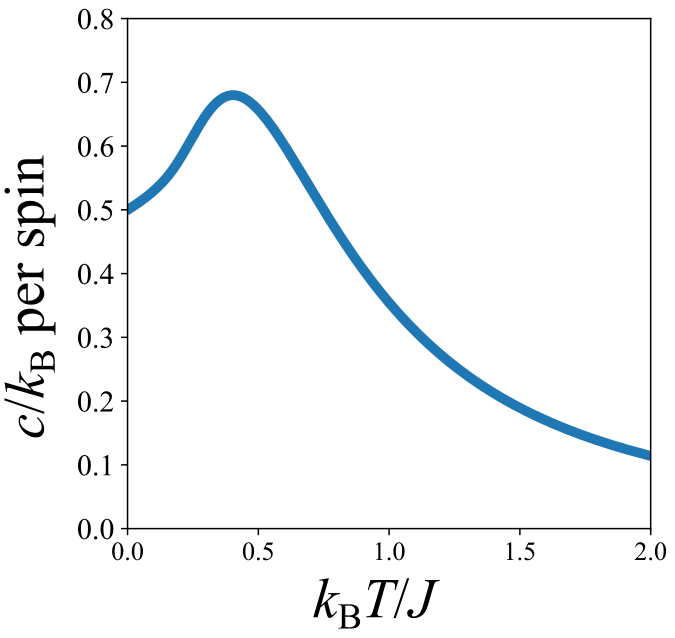
\includegraphics[scale=0.3]{1D_XY_Cv.png}
\caption{Exact specific heat of 1D XY model}
\end{figure}

The most physically interesting cases are the 2 dimensional and the 3 dimensional
ones and they will be discussed in details in the following sections.


\section{2D case}

Phase transitions are classified based on discontinuities of derivatives of the 
free energy, e.g. a ferromagnetic transition is a second-order phase transition 
because it is the magnetic susceptibility, the second derivative of the free energy
with respect of the magnitude of the external field, to be discontinous at the 
critical temperature while the magnetization, the first derivative, is continous.

The 2D case for the XY model is very peculiar because it can be shown to exhibit an
\emph{infinite-order} phase transition called a Kosterlitz-Thouless transition 
after the physicists that first studied it. \footnote{see 
\cite{Kosterlitz_1973}. Thouless and Kosterlitz were awarded the Nobel Prize in 
Physics in 2016 "for theoretical discoveries of topological phase transitions and 
topological phases of matter." 
\url{https://www.nobelprize.org/prizes/physics/2016/summary/}}

The Kosterlitz-Thouless transition consists of a transition between a quasi-ordered 
phase under the critical temperature with a correlation function with a powerlaw
decrease with distance and a disordered phase over the critical temperature with 
a correlation decreasing exponentially with the distance. These kind of order and
disorder states can be shown by identifing vortices in the system. Kosterlitz and 
Thouless gave the following thermodinamical argument to show the existence of such
transition. In the ground state at low temperatures all spins are in the same 
orientation and adding a single vortex will change the entropy of the system by
an amount $\Delta S = k_B \ln(L^2 / a^2)$ where $L$ is the system size, while $a$ 
is the radius of the vortex core. The change in internal energy of the system will
be instead $\Delta E = \pi J \ln(L/a)$. Then the amount of change of free energy will be:
$$ \Delta F = \Delta E - T \Delta S = (\pi J - 2 k_B T) \ln(L/a) $$
At high temperatures (for $\Delta F < 0$) in the thermodinamic limit the system 
will favor the formation of vortices, while viceversa at low temperatures
any vortex will try to annihilate with an antivortex to lower the system energy.
The critical temperature will be the one for which $\Delta F = 0$, so $T_c = \pi
J / 2 k_B$.

Theoritical and Monte Carlo simulation estimates of the critical temperature have
been attempted over the years reaching the well established value of $k_B T_c / J
\simeq 0.88$. Monte Carlo simulations allow also to visualize this kind of 
behaviour using a color map: mapping the spin angles with a colour using a 
continous and periodic color spectrum like a red-green-blue one, where the angle
spans in the interval $[-\pi, \pi)$, the formation of vortex-antivortex pairs can 
be shown at low temperatures as in figure~\ref{fig:kosterlitz}.
\footnote{source 
\url{https://upload.wikimedia.org/wikipedia/commons/7/77/XY_Vortices.svg}}

\begin{figure}[h]
\label{fig:kosterlitz}
\centering
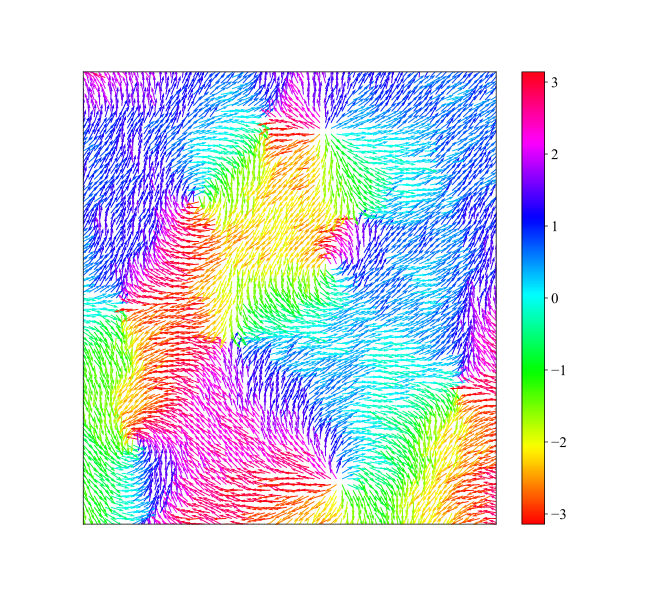
\includegraphics[scale=0.4]{kosterlitz.png}
\caption{Vortex-antivortex formations in 2D XY model at $k_B T / J = 0.4$}
\end{figure}
 

\section{3D case}

In the 3D case (and in higher dimensions) the XY model exhibits a 
ferromagnetic-paramagnetic transition at the critical temperature $k_B T_c / J 
\simeq 2.22$. From a physical point of view this transition plays a central role in
establishing the validity of the model because the values of the so called 
\emph{critical exponents} can be obtained via theoretical means, with quantum
field theory, by experiments and by Monte Carlo simulations.

Critical exponents are a very useful tool used in phase transition description.
They are employed to describe the behavior of physical quantities near the critical
temperature in a huge variety of different systems. They are used in 
\textit{n}-vector model descriptions because it is believed, on strong experimental 
basis, that they do not depend on the particulars of the physical system under
study but only on the following general properties:
\begin{itemize}
  \item the dimension of the system
  \item the dimension of the \emph{spins} considered
  \item the range of interaction
\end{itemize}

The critical exponents are usually denoted by a greek letter and usually the most
important ones are $\alpha$, $\beta$, $\gamma$ and $\delta$. Their meanings will
be explained in the next chapter. 
 
In 3 dimensions, critical exponents can be derived analytically in mean field
theory \footnote{see \url{https://en.wikipedia.org/wiki/Mean-field_theory}}
and experimentally by studying easy-plane magnets and liquid \ce{^{4}He}.




\chapter{Montecarlo simulation}
The XY model has been studied with various approaches, the one taken in this
dissertation is a Monte Carlo simulation that will be implemented to compute
physical observables from which it will be attempted to estimate some critical
exponents. A brief introduction on theory of Monte Carlo simulations will be
followed by a description of this particular implementation and finally the 
results obtained will be illustrated.

\section{Theory}

The main idea of Monte Carlo simulations is to sample a quantity of interest,
treating it as a random variable even if in principal this quantity could be
obtained deterministically. This kind of probabilistic approach, instead of the
deterministic one, becomes useful when the deterministic evaluation via numerical
means results impossible. In physics this usually happens when numerical 
calculations in high dimensions are required, as in evaluation of integrals in 
multiple dimensions, and the computational cost in time scale as $N^2$ or in 
gerenal as a higher power of $N$, with $N$ being the number of dimensions.

Monte Carlo methods are based on the law of large numbers and on the central limit
theorem which states that the expected value of some random variable can be obtained
by the sample mean of indipendent samples of the variable. Then the central problem
of a Monte Carlo algorithm becomes sampling the variables of interest in a
indipendent and representative way.

In phisics and mathematics the algorithm mostly used to accomplish the requirements
needed is the so called Markov chain Monte Carlo sampler. The Markov chain 
\footnote{see \url{https://en.wikipedia.org/wiki/Markov_chain_Monte_Carlo}} is 
constructed based on the target sample distribution and the sampling of the states,
composing the chain, will approach the desired distribution in the limit of an 
infinite chain.

Finally the algorithm that puts all of these concepts togheter is the
Metropolis-Hastings algorithm. \footnote{Check the original work of the Metropolis
spouses and Rosenbluth (\cite{Metropolis1953}) that inspired the invention of the
Metropolis-Hastings algorithm} This algorithm samples any random variable
provided that the probability density function $P(x)$, or a function proportional
to it, is known. Being  based on a Markov chain implicates that every sample is generated
based on the sample generated before, then the sample is accepted or not on 
probabilistic considerations built on $P(x)$. In case the new sample proposal
is rejected, the old sample value is retained and counted as a new sample on which
the values of observables will be computed again.

In the case of a lattice, as in the XY model, starting from a random spins' configuration,
the canonical distribution, coming from canonical ensemble theory, is used to determine which
configuration utilize to compute observables' values. The canonical
distribution is defined as
\begin{equation}
P(\{\sigma_i\}) = \frac{\exp(-\beta H(\{\sigma_i\}))}{Z}
\end{equation}
where $\{\sigma_i\}$ is the spins' configuration and $Z$ is the partition function.

Then in every Metropolis step a new candidate sample is created and the 
probabilities of the configuration are compared using the ratio between them
\begin{equation}
A = \frac{P(\{\sigma_i\}_{mc})}{P(\{\sigma_i\})} = \exp(-\beta (\ H(\{\sigma_i\}_{mc})
- H(\{\sigma_i\})\ ))
\end{equation}
where the $mc$ suffix means the configuration is the Monte Carlo candidate.
Then a random number $\eta$ with a uniformal probability distribution between $0$
and $1$ is picked and the candidate is accepted if $A > \eta$ or rejected viceversa. 

Obtained the new sample (that could easily be the same as the previous one) an observable
value is computed on the configuration. At every step the value of the observable is
saved, and in the end the average over the step values represents the value desired 
and the one comparable with experimental results.

The error on values of the observable cannot only be considered as the standard
deviation of the values computed after every step as these values are not indipendent:
the value from the $n+1$ step follows directly from the value at the $n$ step, therefore
there is an intrinsic correlation between these two. To account for this, correlation
has to be taken in consideration when estimating the uncertainty of the observable.
The correlation of a function $f$ (an observable in this case) is defined as
\begin{equation}
\langle S_L^2 \rangle = \frac{1}{L} \sum_{l=0}^{L} \langle f(x_{i+l}) f(x_i) \rangle
\end{equation}
where $S_L^2$ is an estimate of the correlation, $x_i$ is the step $i$ of the Markov
chain and $L$ is the "maximux" distance in steps in which the correlation is considered
significant. Finally the error on $\langle f \rangle$ will be approximated by 
$\sqrt{S_L^2 - \langle f \rangle^2}$.


\section{Implementation}

The computation of observables values is done in the 3D case, on a cube
of side $L=6$ and periodic boundaries were applied. The atoms in a ferromagnets are
definitely much more than $L^3 = 216$, then the cube under study can be imagined as 
a portion of $216$ atoms in the ferromagnet. These atoms will only interact with other
atoms of the magnet as if they were in an infinite system composed of repeated cubes 
of $216$ atoms. Then periodic boundaries conditions are applied by making interact
the most right atoms with the most left ones, as if another identical cube was
attached on the right of the cube.

Most implementation of the XY model found in higher detailed works usually change one spin
at every Monte Carlo step: obviously this guarantees a higher precision avoiding 
higher fluctations on energy values, but it comes with a very big cost in computation. 
Since the computational power in this case was very limited all of the spin are 
changed at every step guaranteeing a bigger change between a step and another, 
decreasing a lot the correlation between a step and the following one. If the one spin
strategy would have been implemented it would have taken many steps to obtain a 
sufficently different configuration to compute observable values on it.

The amount in change of the angle of the spins is determined by a value usually refered as 
$\Delta$, initialized at $0.1 \degree$. The value of $\Delta$ is the main factor which
controls the amount of correlation between a step and the next one: if $\Delta$ is too
big the candidate configuration will be too different from the original one then most
of the candidate configurations will be discarded and the correlation between steps will
be very high. Something similar happens when $\Delta$ is too little: almost every
candidate configuration will be accepted, but every configuration will still be very
similar from the one before and again the correlation will be very high. Then this
kind of correlation can be minimized by updating the value of $\Delta$ based on the value
of the acceptance ratio: if too many steps are accepted it means $\Delta$ is little,
while in the opposite $\Delta$ will be to big.

% It is known that the Metropolis algorithm risks to be stuck in local minima of energy
% near the critical point, to avoid this from happening an over-relaxation update of the
% configuration has been implemented. This technique consists of changing the value
% of some spins in the configuration to a value of the same energy: the configuration is
% then the same one energetically speaking, but after many steps the system will be able 
% to explore a larger portion of the phase space and will not be stuck in regions near a
% local minimum. The new value of a spin, defined $\mathbf{H}_i \equiv - \sum_{n.n.} \mathbf{s}_j$
% as the local molecular field, is obtained as \footnote{\parencite[see]
% []{Lan}}
% $$ \mathbf{s}_i' = - \mathbf{s}_i + 2 \frac{\mathbf{s}_i \cdot \mathbf{H}_i}{H_i^2}
% \mathbf{H_i} $$
% To avoid form getting a completely different configuration after applying this method
% only one spin every four is updated and only in the temperature region near the 
% critical point.

Since the configurations of interest are the ones in equilibrium, the first $10\text{k}$
steps are used to reach equilibrium and to correct the $\Delta$ to reach an acceptance
ratio in the interval $[0.35,0.65]$. After these $10\text{k}$ steps, other 
$190\text{k}$ steps are performed on which observable values are computed.

The observables computed here are the specifc heat per spin, the magnetization
per spin and are obtained as 
$$ \frac{C_v}{N} = \frac{\langle U^2 \rangle - \langle U \rangle^2}{N (k_B T)^2} $$
$$ \frac{\langle M \rangle}{N} = \frac{1}{N} \big\langle | (\sum_i \cos \theta_i, 
\sum_i \sin \theta_i ) | \big\rangle$$

To compare the values obtained in this work with the ones published before a very simple
and rough estimate of the critical exponents $\alpha$, $\beta$ and $\delta$ is 
performed. Defining $t \equiv (T - T_c)/T_c$ the critical exponents are defined for
magnetic systems as
$$ m \thicksim t^{\beta} \quad (h \rightarrow 0, T < T_c)$$
$$ m \thicksim h^{(1 / \delta)} \quad (h \rightarrow 0, T=T_c)$$
$$ C_v \thicksim t^{-\alpha} \quad  \text{for}\ T > T_c$$
$$\ C_v \thicksim (-t)^{-\alpha} \quad \text{for}\ T < T_c$$

In general $m$ and $h$ are respectively called the \emph{order parameter} and the
\emph{ordering field}. Here $m$ corresponds to the magnetization squared, and $h$ 
corresponds to the magnetic field defined as above. The estimate carried here is
rough because it is simply a fit of the function defined above. Usually much more
sofisticated methods are used such as finite-size scaling methods. \footnote{
see \cite{1988}}

Other critical exponents can be indirectly evalueted using the so called 
\emph{hyperscale relations}. The one of interest are reported below, where $d=3$ 
is the dimension of the system.
\begin{equation}
\label{eq:hyper}
d \nu = 2 - \alpha = 2 \beta + \gamma = \beta(\delta + 1) 
\end{equation}


\section{Results}

In the next pages graphs of the squared magnetization and specific heat in respect of
temperature are shown. It is easy to see the divergence of the specific heat around 
the critical temperature $T_c \simeq 2.22$. As said before a rough attempt 
of estimating the critical temperature and the critical exponents, just by
fitting the functions reported above, will be made.

\begin{figure}[H]
\centering
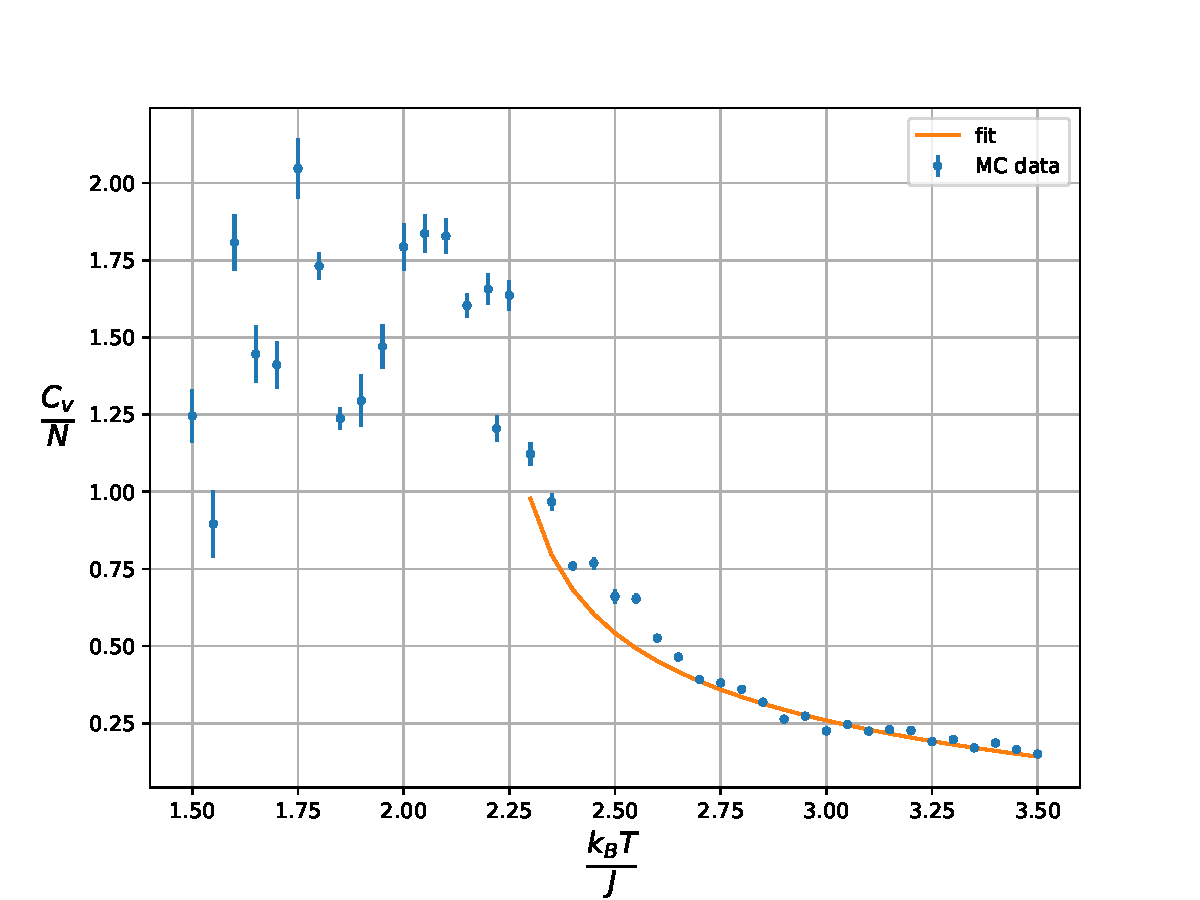
\includegraphics[scale=0.5,page=1]{multipage.pdf}
\caption{$C_v (T)$ for $h=0$}
\end{figure}

\begin{figure}[H]                                   
\centering                                       
\includegraphics[scale=0.5,page=3]{multipage.pdf}
\caption{$M^2 (T)$ for $h=0$}                    
\end{figure}                                     

The roughness of the estimate via simple fit of the functions defining the critical
exponents is due to the fact that the Monte Carlo simulations tend to struggle near critcal
point where observables' values oscillate excessively, reducing then the effectiveness
of the averaging process of the Monte Carlo method. 

\begin{figure}[H]
\centering                                       
\includegraphics[scale=0.5,page=2]{multipage.pdf}
\caption{$C_v (T)$ for $h \neq 0$}                    
\label{fig:cvh}
\end{figure}                                     

Observable values for the ordering field $h\neq 0$ are reported in the graphs below. 
The effect of the field is to keep the order in the spin configuration, raising the
value of the critical point, as can be seen in figure~\ref{fig:cvh}, and to keep
a considerable magnetization after the transistion, as can be see in 
figure~\ref{fig:m2h}.

\begin{figure}[H]
\centering                                       
\includegraphics[scale=0.5,page=4]{multipage.pdf}
\caption{$M^2 (T)$ for $h \neq 0$}                    
\label{fig:m2h}                               
\end{figure}                                     

A study of the magnetization at the critical temperature for different values of the
ordering field is carried to estimate the critical exponent $\delta$. The results are 
reported in figure~\ref{fig:m2hh}.

\begin{figure}[H] 
\centering 
\includegraphics[scale=0.5,page=5]{multipage.pdf}
\caption{$M^2 (h)$ for $T=T_c$}                    
\label{fig:m2hh}
\end{figure}                                     

A table with the results of the fits and the corrisponding critical exponents is
reported below. Theoretical and experimental values for the model are also 
reported. \footnote{for tables of theoretical and experimental values see \cite
{pathria1972statistical}}

\begin{table}[h]
\resizebox{\textwidth}{!}{
\begin{tabular}{|c|c|c|c|c|c|}
\hline
& $\alpha$ & $\beta$ & $\delta$ & $\gamma$ & $\nu$ \\ \hline
Theorical values &  & $0.362 \pm 0.012$ & $4.82 \pm 0.12$ & $1.39 \pm 0.01$ & $0.705 \pm 0.005$ \\ \hline
Experimental values & 0.0-0.2 & 0.3-0.36 & 4.2-4.8 & 4.2-4.8 & 0.62-0.68 \\ \hline
Monte Carlo simulation & $0.201 \pm 0.004$ & $0.438 \pm 0.001$ & $3.86 \pm 0.09$ & $0.654 \pm 0.008$ & $1.08 \pm 0.03$ \\ \hline
$\chi^2_r$ & $\simeq 7\cdot 10^5$ & $\simeq 1\cdot 10^{12}$ & $\simeq 3 \cdot 10^{12}$   &  &    \\ \hline
\end{tabular}}
\end{table}

The values of $\alpha$, $\beta$ and $\delta$ have been obtained directly, while $\gamma$
and $\nu$ have been obtained by $\alpha$, $\beta$ and $\delta$ with the hyperscale
realtions in equation~\ref{eq:hyper}.

By looking at the values of the reduced chi squared it seems obvious that these
fit have to be rejected. Such big values are determined both by an underestimate
of the errors on observables, mainly in the temperature region near the critical 
point, and by a not very good choice of the fitting functions. Anyway a kind of 
agreement, due mainly to the not so precise experimental values, appears beetwen 
experimantal values and the one coming from this work. So it can be said that
the macroscopic behaviour and properties of systems which can be described by the
3 dimensional XY model have been shown.



\chapter{Conclusion}
A theorical analisys of the XY model has been given, starting from its
generalization the n-vector model, simpler cases have been described such as the
Ising model. A detailed theorical study of the 2D and 3D cases for the XY model have been
presented. Monte Carlo simulation theory has been breafly described and has been
put in practice for the 3D case of the XY model. In the last chapter simulation results
have been presented.

The results in the third chapter are not good enough to be compared to other
studies: this is probably due to the fact that near the critical point Monte
Carlo simulations tends not to perform greatly. They tend up to be stuck in
local minima of energy and oscillations in those region of temperature are so high
the averaging process of the algorithm perform much worse than it does in other
regions. This behaviour is known and there exist a few techniques to avoid this
from happening. An example could be the over-relaxation method where the value of
a spin is changed with a different one resulting in the same value of energy: the
sampler will be oblied to sweep more of the phase space and the likelyhood of 
being stuck in a local minimum will decrease significantly. To reduce the
effects of oscillations, averages on slightly different values of temperature
could be taken e.g. the values of observables at $T=2.2$ could be considered 
as the average of the values at $T = 2.195$, $T=2.196$ ... $T=2.205$.\footnote{for
a very detailed work of a Monte Carlo simulation on a GPU for the 3D XY model 
see \cite{Lan}}

All of these technique are generally computational expensive and the limited
equipment did not allow to use them. Anyway in the previous chapters the 
macroscopic behaviour of the XY model has been shown, and even if the values of
critical exponents are not good enough to be considered as a good estimate, 
they are good enough to be compared with some experimental values.




\printbibliography[heading=bibintoc]

\end{document}
